% @Author: bo
% @Date:   2016-05-30 09:35:38
% @Last Modified by:   bo
% @Last Modified time: 2016-06-10 08:47:59

\chapter{综合分类模型}
\label{cha:comprehensiveModal}

\section{综合模型分类结果}
\label{sec:comprehensiveModalResult}

综合第~\ref{cha:fStrategy} 章的多模态融合策略和第~\ref{cha:deeplearning} 章的深度学习方法,我们提出了一个用于分类的多模态融合的综合模型,整体架构如图~\ref{fig:workflow_general} 所示。我们将颜色和深度信息分别作为HMP、CRNN、以及深度学习的输入,提取出特征然后在特征层将不同模态进行融合,最后在方法间使用~\ref{subsec:fBetweenMethod} 小节描述的决策层融合方法进行融合。

% 引入深度学习的意义在于,Deep Learning 在许多方面可以与传统词袋信息提取方法互相补充,有助于突破传统方法的局限。同时,深度学习最终提取出的特征由于。最后,在数据量规模足够大的时候,深度学习能够获得远高于词袋方法的分类及识别准确率。使用深度学习与传统方法互相补充,就好比使用一个新型的、更高精度的传感器与传统的传感器联合做出决策。

\begin{figure}[H] % use float package if you want it here
  \centering
  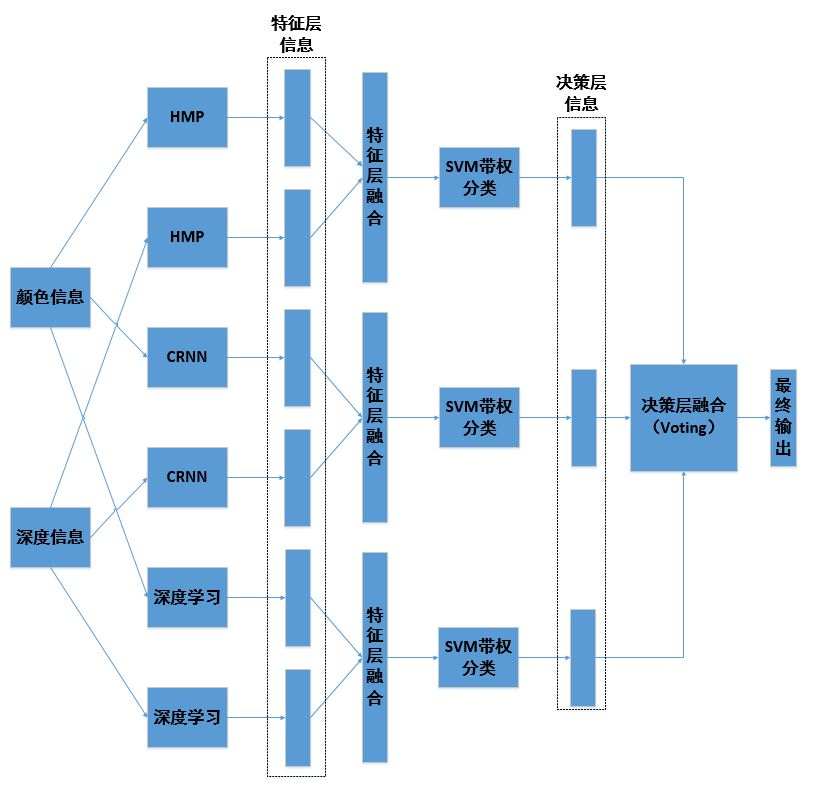
\includegraphics[width=0.9\textwidth]{workflow_general}
  \caption{综合分类模型工作流}
  \label{fig:workflow_general}
\end{figure}

在现有的方法中,传统词袋方法的识别精度不能尽如人意。而深度学习学习虽然准确率较高,但需要大规模数据库的支持。而我们提出的综合分类模型则结合了多种方法的优点:在没有大规模数据库支持时(即表~\ref{tab:cModelResult} 中的FS$^{1}$),深度学习表现一般,但有词袋模型作为准确率的支撑;在有大规模数据库或相关大规模数据库中预训练的模型时(即表~\ref{tab:cModelResult} 中的PM$^{2}$),则深度学习识别的准确率超过传统方法,对最终分类结果可以发挥极大的贡献。
最终模型的识别结果如表~\ref{tab:cModelResult} 所示。
注意由于综合模型中是三方融合,我们还尝试使用了多数投票(Majority Voting)作为融合策略,最终识别结果为91.3\%,略低于我们的带权投票。

\begin{table}[htbp]
  \centering
  \caption{综合模型实验结果}
  \label{tab:cModelResult}
  \begin{minipage}[t]{0.8\textwidth} 
    \begin{tabularx}{\linewidth}{|l|l|X|X|X|}
      \hline
      \multicolumn{2}{|c|}{\diagbox[width=7em]{方法}{模态}} & RGB & Depth & RGB \& Depth\\ \hline
      \multicolumn{2}{|c|}{CRNN}         & $81.7 \pm 1.4$ & $78.9 \pm 1.6$ & $87.6 \pm 1.2$ \\ \hline
      \multicolumn{2}{|c|}{HMP}          & $75.8 \pm 3.4$ & $78.4 \pm 1.9$ & $85.4 \pm 2.6$ \\ \hline
      \multicolumn{2}{|c|}{CRNN \& HMP}  & $83.1 \pm 2.6$ & $82.5 \pm 1.9$ & $89.6 \pm 2.1$ \\ \hline
      \multirow{2}*{深度学习} & FS$^{1}$ & $80.3 \pm 2.6$ & $70.7 \pm 2.3$ & $82.8 \pm 2.4$ \\ \cline{2-5}
                              & PM$^{2}$ & $85.5 \pm 1.5$ & $81.6 \pm 2.8$ & $90.3 \pm 1.8$ \\ \hline
      \multirow{2}*{综合模型} & FS$^{1}$ & $84.1 \pm 2.3$ & $81.9 \pm 2.5$ & $90.1 \pm 1.6$ \\ \cline{2-5}
                              & PM$^{2}$ & $86.9 \pm 1.3$ & $83.8 \pm 2.9$ & $91.6 \pm 1.2$ \\ \hline
    \end{tabularx}\\[2pt]
    \footnotesize
    本表展示的深度信息数据均是经过微调和DAN处理得到的结果,深度学习数据均是采用 fc6 单层信息得到的结果。且方法内均使用~\ref{subsec:fInMethod} 小节描述的特征层融合方法,方法间均使用~\ref{subsec:fBetweenMethod} 小节描述的决策层融合方法。\\
    1:不借助其他数据集从头训练(from scratch)\\
    2:使用在其他数据集上预训练的模型(pretrained model)
  \end{minipage}
\end{table}


各个类的分类准确率如图~\ref{fig:allacc} 所示,可见最终综合模型的百分之八十的类别分类准确率都在百分之九十以上,并且对于大部分类别,综合模型的分类准确率都高于三种方法单独的分类准确率。

不过如果我们重点看最分类准确率最低的十个类(如图~\ref{fig:10worstacc} 所示),可以发现,这些类别分类效果差一方面是因为数据本身问题——三种分类方法准确率都不高;另一方面也是由于分类融合策略在某些类别中被表现较差的方法“拖了后腿”,而没有发挥出表现好的类别的效果。这应该是我们下一步重点探讨的问题。

\begin{figure}[H] % use float package if you want it here
  \centering
  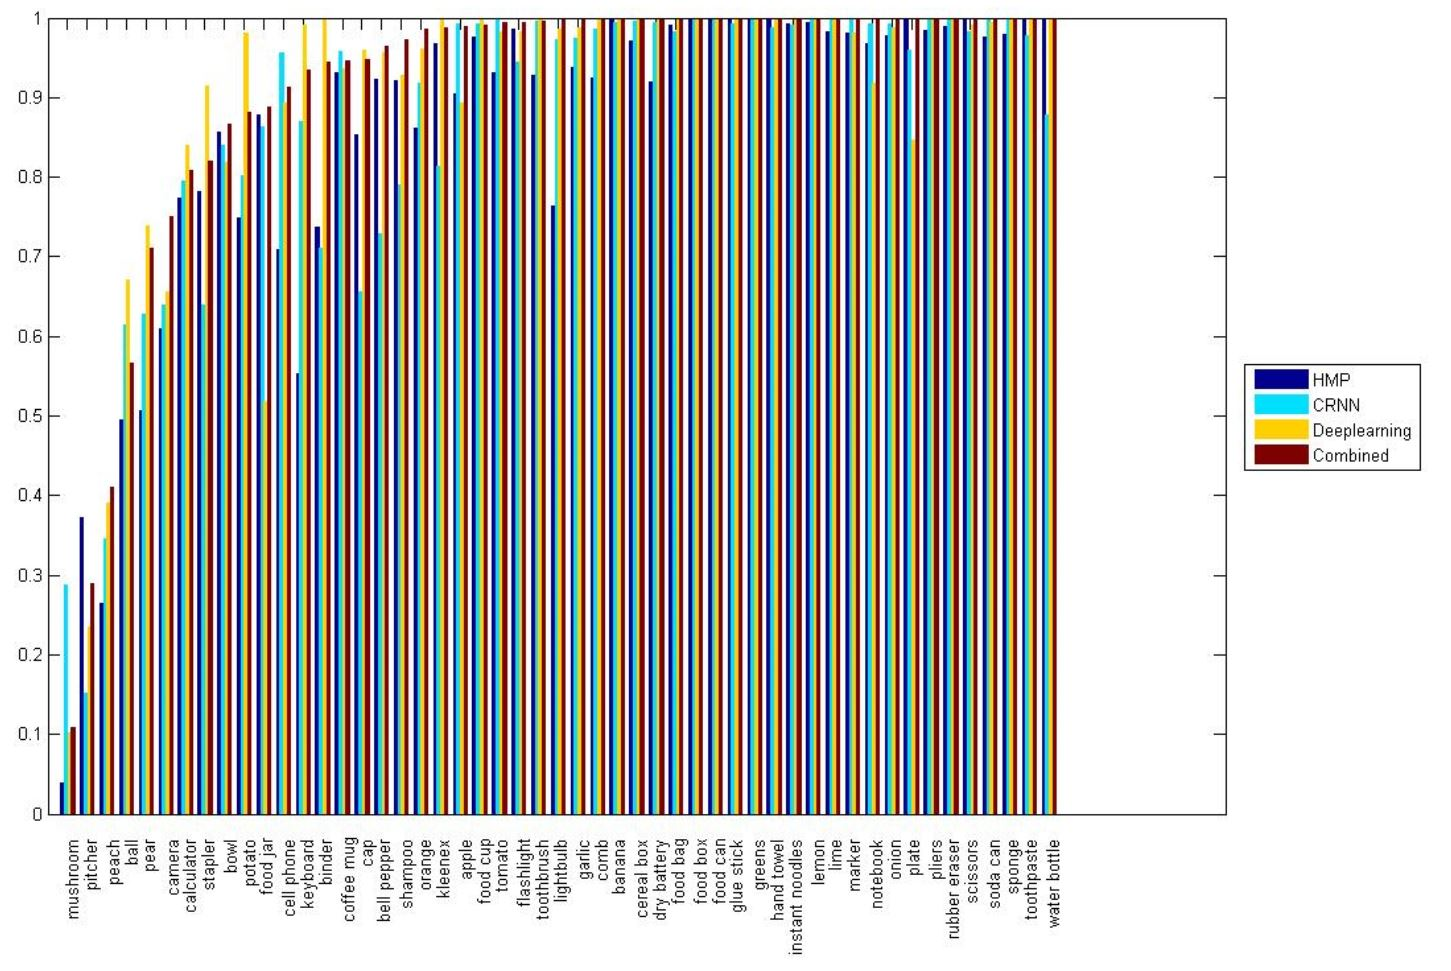
\includegraphics[width=0.95\textwidth]{allacc}
  \caption{分类准确率一览}
  \label{fig:allacc}
\end{figure}

\begin{figure}[H] % use float package if you want it here
  \centering
  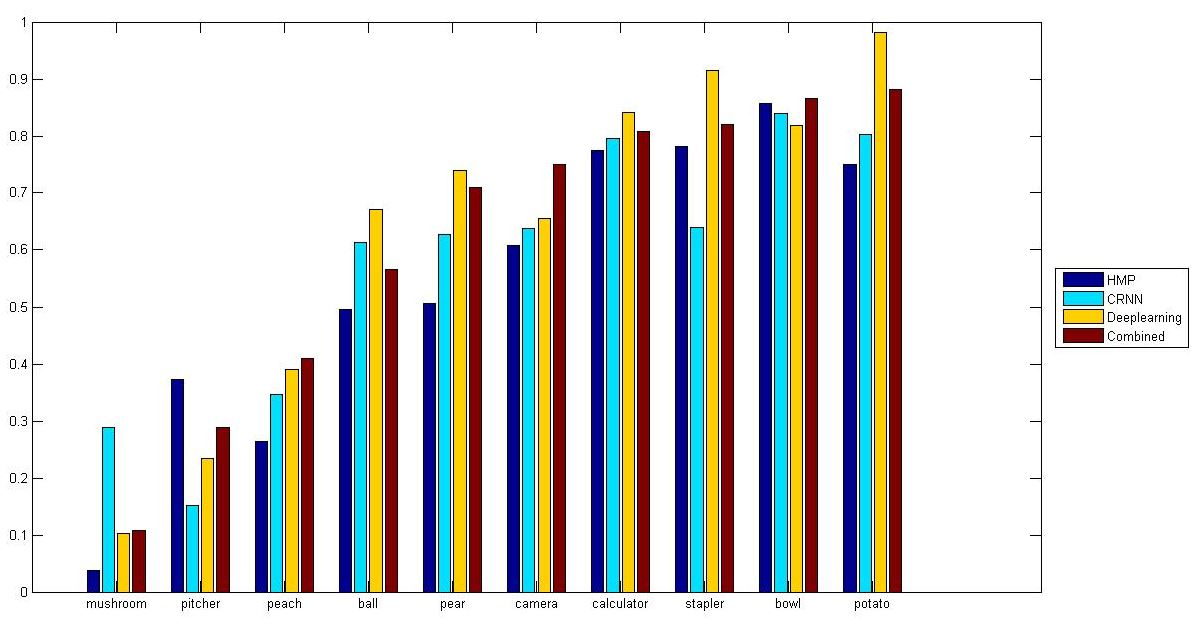
\includegraphics[width=0.95\textwidth]{10worstacc}
  \caption{分类准确率最低的十个类}
  \label{fig:10worstacc}
\end{figure}


\section{多模态识别程序}
\label{sec:demo}

我们按照~\ref{sec:comprehensiveModalResult} 节描述的综合模型实现了具有图形界面的多模态识别实例程序。

程序的流程图如~\ref{fig:workflow_demo} 所示,程序的界面如图~\ref{fig:demo} 所示。在程序开始时会自动载入训练好的 Model ,在识别时可以输入RGB图片和深度图片信息,并选择使用单模态或多模态分类器进行分类。具体分类效果由模型决定,在Qt程序中只做简单的预处理。

\begin{figure}[H] % use float package if you want it here
  \centering
  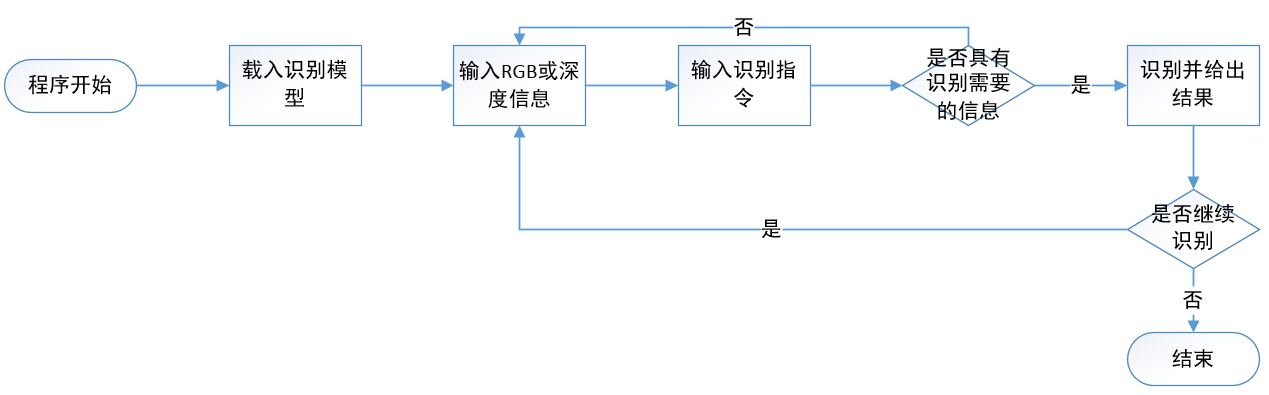
\includegraphics[width=0.95\textwidth]{workflow_demo}
  \caption{多模态识别程序流程图}
  \label{fig:workflow_demo}
\end{figure}

试验平台:
\begin{code}
Windows 8.1
Qt Creator 2.8.1
\end{code}

编译器:
\begin{code}
Qt5.1.1 (MSVC 2010, 32 bit)
GNU Make 3.82.90
Built for i686-w64-mingw32
\end{code}

\begin{figure}[H] % use float package if you want it here
  \centering
  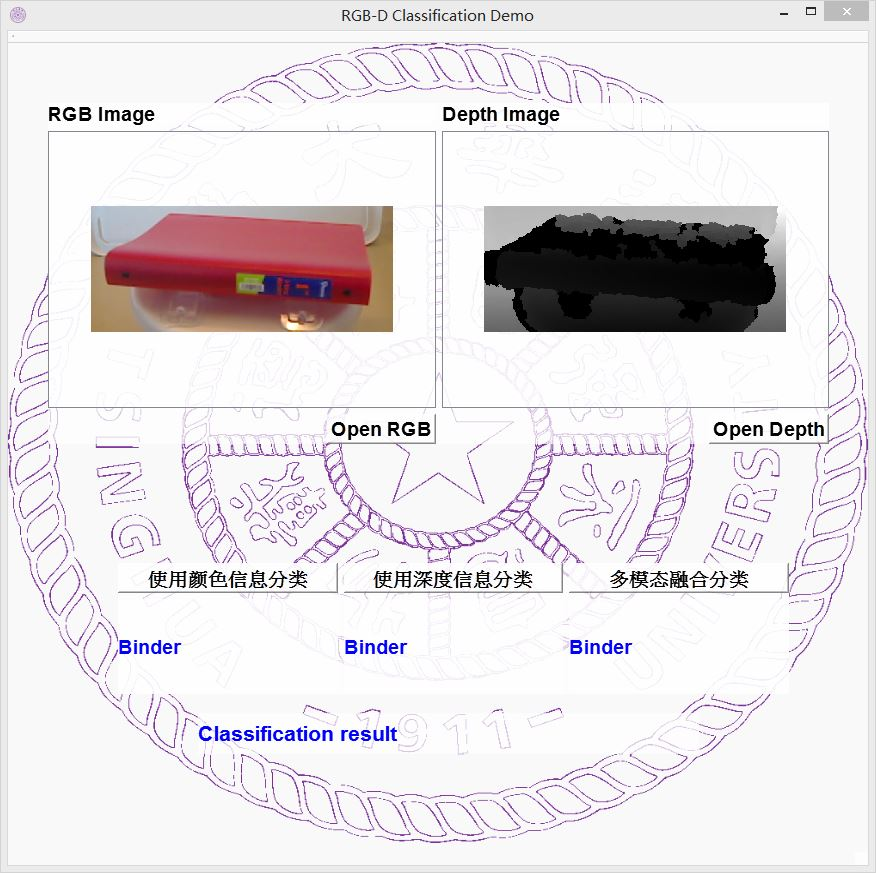
\includegraphics[width=0.95\textwidth]{demo}
  \caption{多模态识别程序界面}
  \label{fig:demo}
\end{figure}
